\iffalse
This file is protected by Copyright. Please refer to the COPYRIGHT file
distributed with this source distribution.

This file is part of OpenCPI <http://www.opencpi.org>

OpenCPI is free software: you can redistribute it and/or modify it under the
terms of the GNU Lesser General Public License as published by the Free Software
Foundation, either version 3 of the License, or (at your option) any later
version.

OpenCPI is distributed in the hope that it will be useful, but WITHOUT ANY
WARRANTY; without even the implied warranty of MERCHANTABILITY or FITNESS FOR A
PARTICULAR PURPOSE. See the GNU Lesser General Public License for more details.

You should have received a copy of the GNU Lesser General Public License along
with this program. If not, see <http://www.gnu.org/licenses/>.
\fi

%----------------------------------------------------------------------------------------
% Required document specific properties
%----------------------------------------------------------------------------------------
\def\comp{fir\_{}complex\_{}sse}
\edef\ecomp{fir_complex_sse}
\def\Comp{FIR Complex SSE}
\def\docTitle{\Comp{} Component Data Sheet}
\def\snippetpath{../../../../../../doc/av/tex/snippets}
%----------------------------------------------------------------------------------------
% Global latex header (this must be after document specific properties)
%----------------------------------------------------------------------------------------
\iffalse
This file is protected by Copyright. Please refer to the COPYRIGHT file
distributed with this source distribution.

This file is part of OpenCPI <http://www.opencpi.org>

OpenCPI is free software: you can redistribute it and/or modify it under the
terms of the GNU Lesser General Public License as published by the Free Software
Foundation, either version 3 of the License, or (at your option) any later
version.

OpenCPI is distributed in the hope that it will be useful, but WITHOUT ANY
WARRANTY; without even the implied warranty of MERCHANTABILITY or FITNESS FOR A
PARTICULAR PURPOSE. See the GNU Lesser General Public License for more details.

You should have received a copy of the GNU Lesser General Public License along
with this program. If not, see <http://www.gnu.org/licenses/>.
\fi

% Sets OpenCPI Version used throughout all the docs. This is updated by
% scripts/update-release.sh when a release is being made and must not
% be changed manually.
\def\ocpiversion{v2.2.0}

\documentclass{article}
\author{}  % Force author to be blank
\date{OpenCPI Release:\ \ \ocpiversion}  % Force date to be blank and override date with version
\title{OpenCPI\\\docTitle}  % docTitle must be defined before including this file
%----------------------------------------------------------------------------------------
% Paper size, orientation and margins
%----------------------------------------------------------------------------------------
\usepackage{geometry}
\geometry{
  letterpaper,  % paper type
  portrait,     % text direction
  left=.75in,   % left margin
  top=.75in,    % top margin
  right=.75in,  % right margin
  bottom=.75in  % bottom margin
}
%----------------------------------------------------------------------------------------
% Header/Footer
%----------------------------------------------------------------------------------------
\usepackage{fancyhdr} \pagestyle{fancy}  % required for fancy headers
\renewcommand{\headrulewidth}{0.5pt}
\renewcommand{\footrulewidth}{0.5pt}
\lhead{\small{\docTitle}}
\rhead{\small{OpenCPI}}
%----------------------------------------------------------------------------------------
% Various packages
%----------------------------------------------------------------------------------------
\usepackage{amsmath}
\usepackage[page,toc]{appendix}  % for appendix stuff
\usepackage{enumitem}
\usepackage{graphicx}   % for including pictures by file
\usepackage{hyperref}   % for linking urls and lists
\usepackage{listings}   % for coding language styles
\usepackage{pdflscape}  % for landscape view
\usepackage{pifont}     % for sideways table
\usepackage{ragged2e}   % for justify
\usepackage{rotating}   % for sideways table
\usepackage{scrextend}
\usepackage{setspace}
\usepackage{subfig}
\usepackage{textcomp}
\usepackage[dvipsnames,usenames]{xcolor}  % for color names see https://en.wikibooks.org/wiki/LaTeX/Colors
\usepackage{xstring}
\uchyph=0  % Never hyphenate acronyms like RCC
\renewcommand\_{\textunderscore\allowbreak}  % Allow words to break/newline on underscores
%----------------------------------------------------------------------------------------
% Table packages
%----------------------------------------------------------------------------------------
\usepackage[tableposition=top]{caption}
\usepackage{float}
\floatstyle{plaintop}
\usepackage{longtable}  % for long possibly multi-page tables
\usepackage{multicol}   % for more advanced table layout
\usepackage{multirow}   % for more advanced table layout
\usepackage{tabularx}   % c=center,l=left,r=right,X=fill
% These define tabularx columns "C" and "R" to match "X" but center/right aligned
\newcolumntype{C}{>{\centering\arraybackslash}X}
\newcolumntype{M}[1]{>{\centering\arraybackslash}m{#1}}
\newcolumntype{P}[1]{>{\centering\arraybackslash}p{#1}}
\newcolumntype{R}{>{\raggedleft\arraybackslash}X}
%----------------------------------------------------------------------------------------
% Block Diagram / FSM Drawings
%----------------------------------------------------------------------------------------
\usepackage{tikz}
\usetikzlibrary{arrows,decorations.markings,fit,positioning,shapes}
\usetikzlibrary{automata}  % used for the fsm
\usetikzlibrary{calc}      % for duplicating clients
\usepgfmodule{oo}          % to define a client box
%----------------------------------------------------------------------------------------
% Colors Used
%----------------------------------------------------------------------------------------
\usepackage{colortbl}
\definecolor{blue}{rgb}{.7,.8,.9}
\definecolor{ceruleanblue}{rgb}{0.16, 0.32, 0.75}
\definecolor{cyan}{rgb}{0.0,0.6,0.6}
\definecolor{darkgreen}{rgb}{0,0.6,0}
\definecolor{deepmagenta}{rgb}{0.8, 0.0, 0.8}
\definecolor{maroon}{rgb}{0.5,0,0}
%----------------------------------------------------------------------------------------
% Define where to hyphenate
%----------------------------------------------------------------------------------------
\hyphenation{Cent-OS}
\hyphenation{install-ation}
%----------------------------------------------------------------------------------------
% Define Commands & Rename Commands
%----------------------------------------------------------------------------------------
\newcommand{\code}[1]{\texttt{#1}}  % For inline code snippet or command line
\newcommand{\sref}[1]{Section~\ref{#1}}  % To quickly reference a section
\newcommand{\todo}[1]{\textcolor{red}{TODO: #1}\PackageWarning{TODO:}{#1}}  % To do notes
\renewcommand{\contentsname}{Table of Contents}
\renewcommand{\listfigurename}{List of Figures}
\renewcommand{\listtablename}{List of Tables}

% This gives a link to gitlab.io document. By default, it outputs the filename.
% You can optionally change the link, e.g.
% \githubio{FPGA\_Vendor\_Tools\_Installation\_Guide.pdf} vs.
% \githubio[\textit{FPGA Vendor Tools Installation Guide}]{FPGA\_Vendor\_Tools\_Installation\_Guide.pdf}
% or if you want the raw ugly URL to come out, \githubioURL{FPGA_Vendor_Tools_Installation_Guide.pdf}
\newcommand{\githubio}[2][]{% The default is for FIRST param!
\href{http://opencpi.gitlab.io/releases/\ocpiversion/docs/#2}{\ifthenelse{\equal{#1}{}}{\texttt{#2}}{#1}}}
\newcommand{\gitlabcom}[2][]{% The default is for FIRST param!
\href{http://gitlab.com/opencpi/#2}{\ifthenelse{\equal{#1}{}}{\texttt{#2}}{#1}}}
\newcommand{\githubioURL}[1]{\url{http://opencpi.gitlab.io/releases/\ocpiversion/docs/#1}}
% Lastly, if you want a SINGLE leading path stripped, e.g. assets/X.pdf => X.pdf:
\newcommand{\githubioFlat}[1]{%
\StrBehind{#1}{/}[\den]%
\href{http://opencpi.gitlab.io/releases/\ocpiversion/docs/#1}{\texttt{\den}}%
}
%----------------------------------------------------------------------------------------
% VHDL Coding Language Style
% modified from: http://latex-community.org/forum/viewtopic.php?f=44&t=22076
%----------------------------------------------------------------------------------------
\lstdefinelanguage{VHDL}
{
  basicstyle=\ttfamily\footnotesize,
  columns=fullflexible,keepspaces,  % https://tex.stackexchange.com/a/46695/87531
  keywordstyle=\color{ceruleanblue},
  commentstyle=\color{darkgreen},
  morekeywords={
    library, use, all, entity, is, port, in, out, end, architecture, of,
    begin, and, signal, when, if, else, process, end,
  },
  morecomment=[l]--
}
%----------------------------------------------------------------------------------------
% XML Coding Language Style
% modified from http://tex.stackexchange.com/questions/10255/xml-syntax-highlighting
%----------------------------------------------------------------------------------------
\lstdefinelanguage{XML}
{
  basicstyle=\ttfamily\footnotesize,
  columns=fullflexible,keepspaces,
  morestring=[s]{"}{"},
  morecomment=[s]{!--}{--},
  commentstyle=\color{darkgreen},
  moredelim=[s][\color{black}]{>}{<},
  moredelim=[s][\color{cyan}]{\ }{=},
  stringstyle=\color{maroon},
  identifierstyle=\color{ceruleanblue}
}
%----------------------------------------------------------------------------------------
% DIFF Coding Language Style
% modified from http://tex.stackexchange.com/questions/50176/highlighting-a-diff-file
%----------------------------------------------------------------------------------------
\lstdefinelanguage{diff}
{
  basicstyle=\ttfamily\footnotesize,
  columns=fullflexible,keepspaces,
  breaklines=true,                            % wrap text
  morecomment=[f][\color{ceruleanblue}]{@@},  % group identifier
  morecomment=[f][\color{red}]-,              % deleted lines
  morecomment=[f][\color{darkgreen}]+,        % added lines
  morecomment=[f][\color{deepmagenta}]{---},  % Diff header lines (must appear after +,-)
  morecomment=[f][\color{deepmagenta}]{+++},
}
%----------------------------------------------------------------------------------------
% Python Coding Language Style
%----------------------------------------------------------------------------------------
\lstdefinelanguage{python}
{
  basicstyle=\ttfamily\footnotesize,
  columns=fullflexible,keepspaces,
  keywordstyle=\color{ceruleanblue},
  commentstyle=\color{darkgreen},
  stringstyle=\color{orange},
  morekeywords={
    print, if, sys, len, from, import, as, open,close, def, main, for, else,
    write, read, range,
  },
  comment=[l]{\#}
}
%----------------------------------------------------------------------------------------
% Fontsize Notes in order from smallest to largest
%----------------------------------------------------------------------------------------
%    \tiny
%    \scriptsize
%    \footnotesize
%    \small
%    \normalsize
%    \large
%    \Large
%    \LARGE
%    \huge
%    \Huge

\graphicspath{{figures/}}
%----------------------------------------------------------------------------------------

\begin{document}
\maketitle
\thispagestyle{empty}
\newpage

\begin{center}
	\textit{\textbf{Revision History}}
		\begin{table}[H]
		\label{table:revisions} % Add "[H]" to force placement of table
			\begin{tabularx}{\textwidth}{|c|X|l|}
			\hline
			\rowcolor{blue}
			\textbf{Revision} & \textbf{Description of Change} & \textbf{Date} \\
		    \hline
		    v1.4 & & 10/2018 \\
		    \hline
       	 	v1.5 &  & 4/2019 \\
		    \hline
		     v1.6 & Converted Worker to version 2 & 11/2019 \\
		    \hline
			\end{tabularx}
		\end{table}
\end{center}	
\newpage

\def\name{\comp}
\def\workertype{Application}
\def\version{\ocpiversion}
\def\releasedate{11/2019}
\def\componentlibrary{ocpi.assets.dsp\_{}comps}
\def\workers{\comp{}.hdl}
\def\testedplatforms{alst4, isim, Matchstiq-Z1(PL), ml605, modelsim, xsim, ZedBoard(PL)}
\section*{Summary - \Comp}
\begin{tabular}{|c|M{13.5cm}|}
  \hline
  \rowcolor{blue}
   & \\
  \hline
  Name              & \comp             \\
  \hline
  Worker Type       & \workertype       \\
  \hline
  OpenCPI Release   & \ocpiversion      \\
  \hline
  Last Update       & \releasedate      \\
  \hline
  Component Library & \componentlibrary \\
  \hline
  Workers           & \workers          \\
  \hline
  Tested Platforms  & \testedplatforms  \\
  \hline
\end{tabular}


\section*{Functionality}
\begin{flushleft}
	The FIR Complex SSE (Systolic Symmetric Even) component inputs complex signed samples and filters them based upon a programmable number of coefficient tap values. The underlying FIR Filter implementation makes use of a symmetric systolic structure to construct a filter with an even number of taps and symmetry about its midpoint.
\end{flushleft}

\section*{Worker Implementation Details}
\subsection*{\comp.hdl}
\subsubsection*{Filter taps}
\begin{flushleft}
	The \verb+NUM_TAPS_p+ parameter determines the length of the \verb+taps+ property.  Each 16-bit tap within the \verb+taps+ property is truncated by taking the \verb+COEFF_WIDTH_p+ number of least significant bits. Care should be taken to ensure that the \verb+COEFF_WIDTH_p+ parameter is $\le$ 16. The most significant bit of the truncated value is used as a sign bit. The truncated data is formatted as QN.0, where N is \verb+COEFF_WIDTH_p+-1. The truncated taps are effectively the first half of all coefficients used to perform convolution. The last half is equivalent to the reverse-indexed copy of the first half, allowing the coefficients to have symmetry about their midpoint. This symmetry of FIR coefficients results in group delay being constant across all frequencies.
\medskip
\end{flushleft}

\subsection*{Filter function}
\begin{flushleft}

	This implementation uses \verb+NUM_TAPS_p+ multipliers per each input rail to process input data at the clock rate - i.e. this worker can handle a new input value every clock cycle. It is unnecessary to round the output data from this filter at the worker level because it is already being done within the macc\_systolic\_sym primitive.\medskip

	The FIR Complex SSE worker utilizes the OCPI \textit{iqstream\_protocol} for both input and output ports. The \textit{iqstream\_protocol} defines an interface of 16-bit complex signed samples. The \verb+DATA_WIDTH_p+ parameter may be used to reduce the FIR Complex SSE hdl worker's internal data width to less than 16-bits.
\end{flushleft}
{\centering\captionsetup{type=figure}\includegraphics[scale=0.65]{fir_systolic_sym_even}\par\captionof{figure}{FIR Complex SSE Block Diagram - 8-tap example per I/Q rail}\label{fig:circuit}}

\section*{Theory}
\begin{flushleft}
	This filter will produce valid outputs one clock after each valid input, but care must be exercised when attempting to align outputs according to the filter's actual group delay and propagation delay.\medskip

	For a FIR filter with symmetric impulse response we are guaranteed to have linear phase response and thus constant group delay vs. frequency. In general, the group delay will be equal to (N-1)/2, where N is the number of filter taps.	The filter topology itself will add some propagation delay to the response. For this design the total delay from an impulse input to the beginning of the impulse response will be \verb+NUM_TAPS_p+ + 4 samples.
\end{flushleft}

\section*{Block Diagrams}
\subsection*{Top level}
\begin{center}
	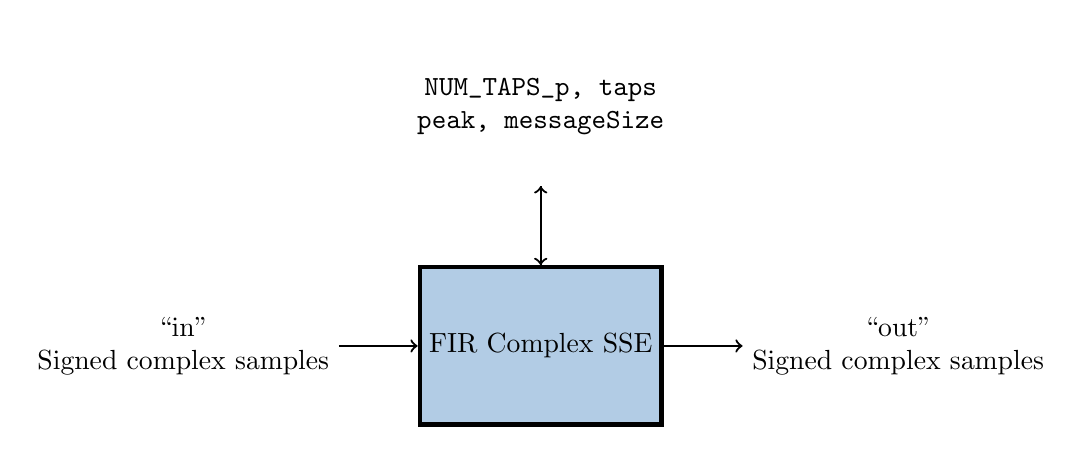
\begin{tikzpicture}[% List of styles applied to all, to override specify on a case-by-case
			every node/.style={
				align=center,  		% use this so that the "\\" for line break works
				minimum size=2cm	% creates space above and below text in rectangle
			},
			every edge/.style={draw,thick}
		]
		\node[rectangle,ultra thick,draw=black,fill=blue](R2){\Comp};
		\node[rectangle,draw=white,fill=white](R3)[left= of R2]{``in'' \\ Signed complex samples};
		\node[rectangle,draw=white,fill=white](R4)[right= of R2]{``out'' \\ Signed complex samples};
		\node[rectangle,draw=white,fill=white](R5)[above= of R2]{\verb+NUM_TAPS_p, taps+ \\ \verb+peak, messageSize+};
		\path[->]
		(R3)edge []	node [] {} (R2)
		(R2)edge []	node [] {} (R4)
		(R2)edge []	node [] {} (R5)
		(R5)edge []	node [] {} (R2)
		;
	\end{tikzpicture}
\end{center}

\newpage

\section*{Source Dependencies}
\subsection*{\comp.hdl}
\begin{itemize}
	\item projects/assets/components/dsp\_comps/fir\_complex\_sse.hdl/fir\_complex\_sse.vhd
          \input{snippets/FIR_Complex_SSE_Primitive_Dependencies}
\end{itemize}

\begin{landscape}
	\section*{Component Spec Properties}
	\begin{scriptsize}
		\begin{tabular}{|p{1.5cm}|p{1cm}|c|c|c|p{3cm}|c|p{7cm}|}
			\hline
			\rowcolor{blue}
			Name               & Type   & SequenceLength & ArrayDimensions   & Accessibility       & Valid Range                                                                      & Default & Usage                                                                        \\
			\hline
			\verb+NUM_TAPS_p+  & UChar  & -              & -                 & Parameter & 1-?                                                                              & 16      & Half the number of coefficients used by each real/imag even symmetric filter \\
			\hline
			\verb+peak+        & Short  & -              & -                 & Volatile            & Standard                                                                         & 0       &   Peak value of I/Q output (valid when PEAK\_MONITOR = true)                 \\
			\hline
			\verb+messageSize+ & UShort & -              & -                 & Writable  & 8192                                                                             & 8192    & Number of bytes in output message (Not implemented by Version 2)  \\
			\hline
			\verb+taps+        & Short  & -              & \verb+NUM_TAPS_p+ & Initial  & -2\textsuperscript{COEFF\_WIDTH\_p-1} to +2\textsuperscript{COEFF\_WIDTH\_p-1}-1 & -       & Symmetric filter coefficient values loaded into both real/imag filters       \\
			\hline
		\end{tabular}
	\end{scriptsize}

	\section*{Worker Properties}
	\subsection*{\comp.hdl}
	\begin{scriptsize}
		\begin{tabular}{|p{3cm}|p{2cm}|p{1cm}|c|c|c|c|c|p{5cm}|}
			\hline
			\rowcolor{blue}
			Type     & Name                 & Type  & SequenceLength & ArrayDimensions & Accessibility       & Valid Range & Default & Usage                                        \\
			\hline
			Property & \verb+DATA_WIDTH_p+  & UChar & -              & -               & Parameter & 1-16        & 16      & Data Width of I and Q for internal processing \\
			\hline
			Property & \verb+COEFF_WIDTH_p+ & UChar & -              & -               & Parameter & 1-32        & 16      & Coefficient width in bits.                 \\
			\hline
			Property & \verb+PEAK_MONITOR+ & bool & -              & -               & Parameter &  -       & true      & Enable/Disable build-time inclusion of Peak Monitoring                            \\
			\hline
		\end{tabular}
	\end{scriptsize}


	\section*{Component Ports}
	\begin{scriptsize}
		\begin{tabular}{|M{2cm}|M{1.5cm}|M{4cm}|c|c|M{9cm}|}
			\hline
			\rowcolor{blue}
			Name & Producer & Protocol           & Optional & Advanced & Usage                  \\
			\hline
			in   & false    & iqstream\_protocol & false    & -        & Complex signed samples \\
			\hline
			out  & true     & iqstream\_protocol & false    & -        & Complex signed samples \\
			\hline
		\end{tabular}
	\end{scriptsize}

	\section*{Worker Interfaces}
	\subsection*{\comp.hdl}
	\begin{scriptsize}
		\begin{tabular}{|M{2cm}|M{1.5cm}|c|c|M{12cm}|}
			\hline
			\rowcolor{blue}
			Type            & Name & DataWidth & Advanced                & Usage                  \\
			\hline
			StreamInterface & in   & 32        & - & Signed complex samples \\
			\hline
			StreamInterface & out  & 32        & InsertEOM=1 & Signed complex samples \\
			\hline
		\end{tabular}
	\end{scriptsize}
\end{landscape}

\section*{Control Timing and Signals}
\begin{flushleft}
	The FIR Complex SSE worker uses the clock from the Control Plane and standard Control Plane signals. The Raw Property interface is used to read/write coefficient values.
\end{flushleft}

\begin{landscape}
\section*{Worker Configuration Parameters}
\subsubsection*{\comp.hdl}
%\input{../../\ecomp.hdl/configurations.inc}
\section*{Performance and Resource Utilization}
\subsubsection*{\comp.hdl}
%\input{../../\ecomp.hdl/utilization.inc}
\end{landscape}

\section*{Test and Verification}


\begin{flushleft}
A single test case is implemented to validate the FIR Complex SSE component. The python script \textit{gen\_lpf\_taps.py} is used to generate a taps file consisting of \verb+NUM_TAPS_p+ filter coefficients. Input data is generated by first creating a *.dat input file consisting of a single maximum signed value of +32767 (for each real/imag filter) followed by 2*(\verb+NUM_TAPS_p+-1) zero samples (again for each real/imag filter). The *.bin input file is the binary version of the *.dat ASCII file repeated 2*\verb+NUM_TAPS_p+ times.\medskip

The FIR Complex SSE worker inputs complex signed samples, filters the input as defined by the coefficient filter taps, and outputs complex signed samples. Since the input consists of an impulse response - that is, a maximal `one' sample followed by all zeros equal to the length of the filter - the output of each filter is simply the coefficient values.\medskip

For verification, the output file is first checked that both I and Q outputs match. Then the I output rail is compared against the taps file, and finally the Q output rail is also compared against the taps file. A $\pm1$ difference is allowed in value while comparing output rails against the filter coefficient values. Figures \ref{fig:out_time} and \ref{fig:out_freq} depict the filtered results of the impulse input.
\end{flushleft}

	\begin{figure}[ht]
		\centering
		\begin{minipage}{.5\textwidth}
			\centering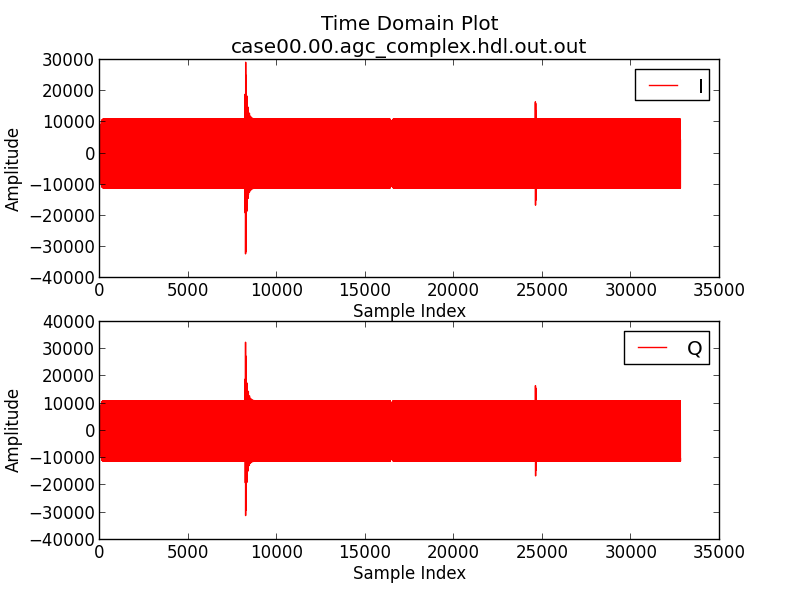
\includegraphics[width=1.0\linewidth]{output_time}
			\captionof{figure}{Time Domain Impulse Response}
			\label{fig:out_time}
		\end{minipage}%
		\begin{minipage}{.5\textwidth}
			\centering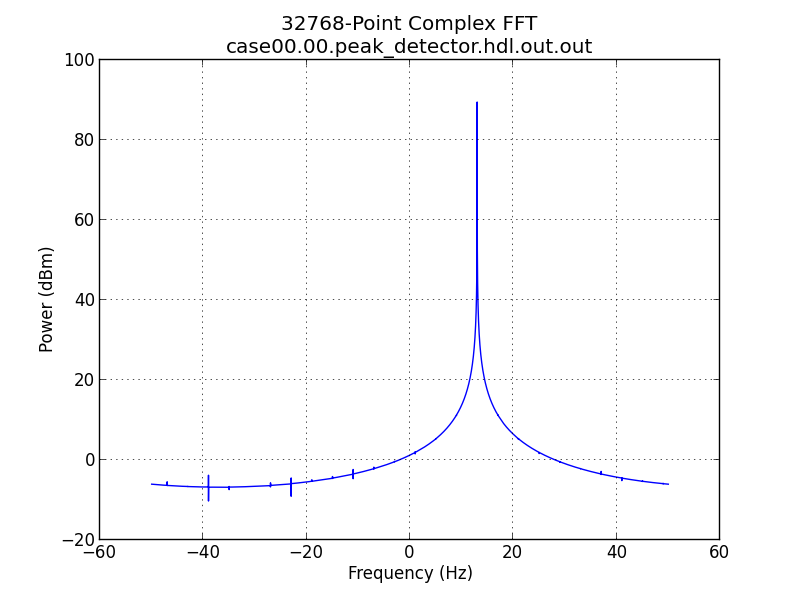
\includegraphics[width=1.0\linewidth]{output_freq}
			\captionof{figure}{Frequency Domain Impulse Response}
			\label{fig:out_freq}
		\end{minipage}
	\end{figure}
\end{document}
